\chapter{\label{ax:a-michele_sambin_videoloop}Michele Sambin's \textit{Videoloop}}

The first and the main case study in this PhD research focuses on the reactivation and conservation of a series of analogue video artworks from the 1970s, created using the \textit{videoloop} technique developed by artist Michele Sambin. This case study was especially important for testing and optimising the \textit{Multilevel Dynamic Conservation} (MDC), the CATTA reactivation workflow, and the \textit{Baalman Visual Language} (BVL), as well as their application in the graph database Neo4j. The artworks underwent multiple iterations, with changes and technological updates from their original analogue form.

\section{Objectives}
The main objectives of this case study, in addition to the application, testing and refinement of the systems introduced in Chapter~\ref{ch:3-mdc_model-reactivation_workflow-instruction_template}, are:
\begin{enumerate}
    \item to explore the role of artists in both technology development and conservation processes;
    \item to study oral history: interview with the artist;
    \item to apply the reactivation through analog-to-digital migration;
    \item to create a Neo4j database according to the MDC model–see Chapter~\ref{ch:4-madc_model_application} for more details.
\end{enumerate}

Il ruolo degli artisti nei processi di sviluppo tecnologico
collaborazione con gli artisti nella conservazione
riattivazione per mezzo di migrazione analogico-digitale
inclusione della Oral history: intervista all'artista

\section{Introduction}
Michele Sambin is a versatile Italian artist who has worked with painting, film, video art, music, and theatre since the 1960s. Technology has always been a key part of his work as an artistic tool. One of Sambin's traits is his experimentation with simple, well-known technologies instead of new and advanced ones. He creates original forms of creative expression by pushing these familiar technologies to their limits. Some examples are the innovative use of the real-time audio-video recording in the 1970s, which led to the development of the \textit{videoloop} technique (discussed in detail in this chapter); the use of digital drawing tablets and Photoshop to interact with stages’ proscenium, which led to the \textit{light painting} technique (in Figure~\ref{fig:aa-light_painting} a photo with the visual effect produced with the technique).\\
\begin{figure}[!h]
    \centering
    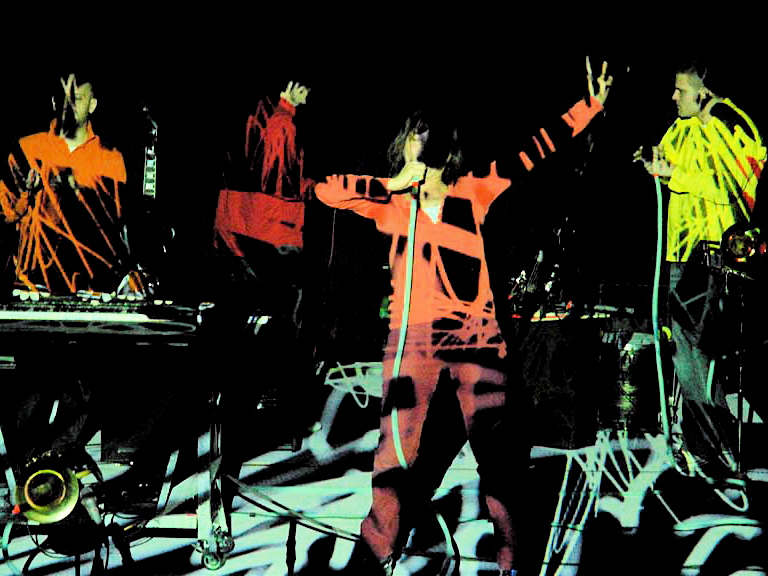
\includegraphics[width=\linewidth]{chapters/appendix/a/image/figa-lightpainting.jpg}
    \caption{A photo from \textit{Tutto è vivo} (2008), a production by Michele Sambin with TAM, where the artist used the \textit{light painting} technique.}
    \label{fig:aa-light_painting}
\end{figure}
Sambin is generally known for his innovative work in multimedia experimental theatre. He has recently been notably recognised for his audiovisual performances, which form a fundamental part of his artistic production.\\
Sambin’s theatrical works with the Italian company TAM Teatromusica –which he co-founded– are especially notable. He created and co-created over 40 original productions with TAM that combined live performance with experimental music and video. The first production with TAM was \textit{Armoniche} (1980), where four performers interacted with video projections while playing harmonicas, creating a spatial sound experience. It was with TAM that Sambin developed the \textit{light painting} technique, which was featured in productions like \textit{Musica senza musicisti} (2004), \textit{Squarcione} (2004), \textit{Lux} (2006), and especially \textit{Tutto è vivo} (2008).\\ 
Sambin gained widespread recognition only for his theatre work until the early 2000s. However, with renewed interest in Italian video art in the late 1990s, scholars and experts began to rediscover his earlier experimental film and video art pieces from the 1960s and 70s. These include experimental films such as \textit{Anamnesi} (1968), \textit{1 e 2} (1969), \textit{Blu d'acqua} (1972), \textit{Film a strisce} (1976), and others. And performative video artwork, such as \textit{Spartito per violoncello} (1974), \textit{Concerto per clarino e VTR} (1976), \textit{Autoritratto} (1977), and \textit{VTR\&I} (1978). His \textit{videoloop} technique emerged with this last piece and  \textit{Il tempo consuma} (1978), and it was later used in works like \textit{Anche le mani invecchiano} (1979), \textit{Sax} (1980), \textit{Io mi chiamo Michele} (1980), and many others.\\
Today, the \textit{videoloop} technique and Sambin’s video art performances are considered significant works in Italian video art history, as we can read in many sources (a monographic book \cite{lischi2014michele}; many papers about Sambin’s multimedia art \cite{leuzzi2019re, d2021invenzioni, gallo2021intimacy}, among others; a project about Italian video art, \textit{REWINDItalia} \cite{Leuzzi2015-bh}; a monographic exhibition \cite{dimarino2022silvana}; and a Italian video art exhibition \cite{saba2022videoarte}). 

\subsection*{Videoloop technique}
\begin{quote}
    "The videoloop technique was born as a meeting between the desire to work with the video in real-time and, as often happens, an accidental element. It all started with the fact that inside the open-reel tape package (normally used at the time), I found a piece of duct tape used to repair a cut" \cite{fiordelmondo2023toward}.
\end{quote}
The small piece of duct tape sparked a series of inspirations and connections for the artist. It reminded him of his earlier work with audio tape alongside Teresa Rampazzi, Terry Riley's audio loop technique—where two Revox tape recorders were placed five meters apart, connected by a tape—and his early video experiments. All these ideas came together, leading to the creation of the first \textit{videoloop} in 1978.\\
The \textit{videoloop} is a circular system created by two video recorders with a closed ring tape. The closed ring tape is made through the conjunction of tape extremities. The artist explains the technique as follows: 
\begin{quote}
    "The closed ring tape scrolls between two video recorders which are placed at a specific distance to keep the tape under tension. The tape is dragged by the video recorders’ engines and it spins. The first video recorder works as a recorder, while the second works as a player. The camera placed in front of the monitor is attached to the first video recorder, and the second video recorder is attached to the monitor"\footnote{Translation into English by the author.} \cite{lischi2014michele}. 
\end{quote}
Figure~\ref{fig:aa-videoloop_graph01} shows a graphical representation of the system. With this technique, Sambin finds a way to overlap and accumulate video and sound material endlessly. The artist records himself at regular intervals and interacts with the playback material, becoming the interlocutor of his electronic self \cite{balzola2019arti}.
\begin{figure}[!h]
    \centering
    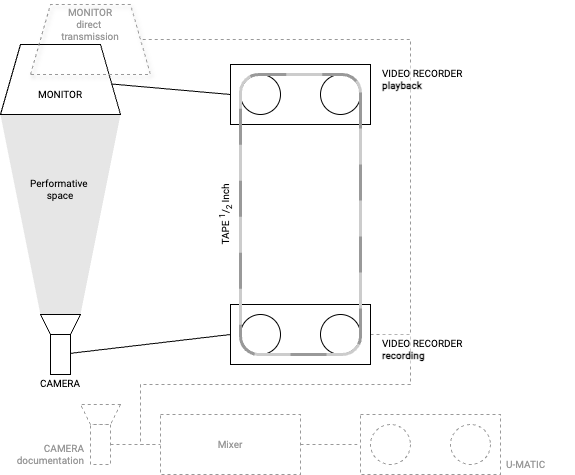
\includegraphics[width=\linewidth]{chapters/appendix/a/image/grapha-videoloop01.png}
    \caption{Graphical representation of the original analogue \textit{videoloop}.}
    \label{fig:aa-videoloop-graph01}
\end{figure}
With this technique, Michele Sambin created many video art performance pieces. One of the first and most relevant one, \textit{Il tempo consuma} (1978), was performed live just once at Fondazione Bevilacqua La Masa in Venice in 1979. It was also exhibited at the \textit{Camere Incantate} exhibition at the Royal Palace in Milan in 1980, but it was not live. As explained by the artist:\\ 
\begin{quote}
    At the end of the seventies, the excitement for new forms of live performance was slightly declining. The same thing happened to pioneering video art, which was considered no longer of interest” \cite{fiordelmondo2023toward}.
\end{quote}
For these reasons, the works with the \textit{videoloop} didn’t obtain significant feedback for many years, and Sambin was considered mainly for his theatrical works. However, as the artist stated in the documentary film \textit{Più della vita} (2019) by Raffella Rivi and in an interview created explicitly in the context of this case study \cite{fiordelmondo2023toward},  the videoloop is one of the most relevant techniques in his artistic production, which has affected all his subsequent work.

\section{Reactivation}
The reactivation process began in May 2021 and went through five different interactions until October 2024. Although it mainly focused on the performance of \textit{Il tempo consuma}, it also comprehends other historical pieces made with the \textit{videoloop} technique and new experimentations. The reactivation was done using the CATTA reactivation workflow and the MDC models (explained in Chapter~\ref{ch:3-mdc_model-reactivation_workflow-instruction_template}). The process of reactivation was conducted by the author alongside the artist. Each choice was made through an interdisciplinary comparison between the aesthetic aspects emphasised by the artist and the development approaches presented by the research group.

\subsection*{Collection}
The first step was to gather the first \textit{Iteration Files} (IFs) regarding the first performances in the late 1970s and early 1980s by collecting \textit{bit}s, \textit{data}, and \textit{experience} documents. The biggest challenge during reactivation was defining the first type of item (\textit{bit}) since the original system used in the first performance had not been preserved. The original equipment—analogue video recorders, cameras, cathode-ray tube monitors, and tape—was no longer available because the artist didn’t own it. As a result, the \textit{bit}s of the IFs for the first performance and exhibition remain incomplete. However, we could create a partial metadata description for the missing \textit{bit}s based on bibliographic documentation.\\
Collecting the \textit{data} and \textit{experience} documents, however, was much more manageable. Sambin has always paid attention to documenting his works by creating sketches and scores with detailed comments and instructions, all of which are considered part of the IF’s \textit{data}. There are also several \textit{experience}-type items. The artist made audiovisual recordings (a screenshot of the video can be seen in Figure~\ref{fig:aa-iltempoconsuma01}) and took photos of the performance, capturing the original setup, the actions, the placement of tools, and the use of technology.
\begin{figure}[!h]
    \centering
    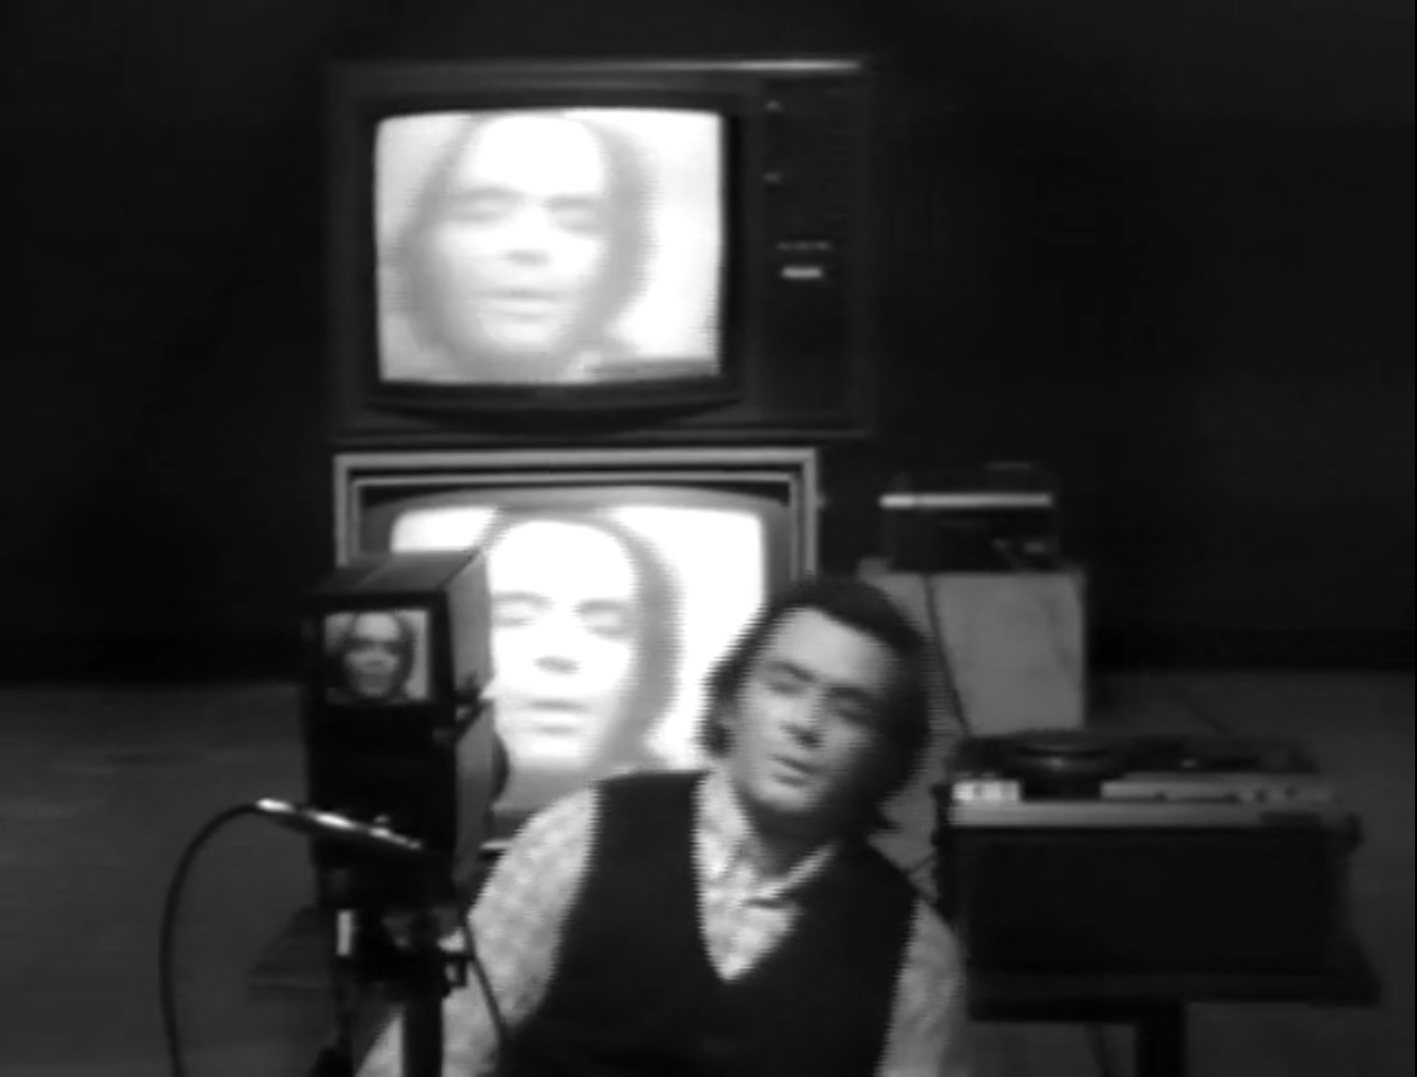
\includegraphics[width=\linewidth]{chapters/appendix/a/image/figa-iltempoconsuma.jpg}
    \caption{Screenshot of the 1978 audiovisual documentation of \textit{Il tempo consuma}.}
    \label{fig:aa-iltempoconsuma01}
\end{figure}
Moreover, we gathered various bibliography items related to Michele Sambin’s video art, such as those mentioned above \cite{lischi2014michele, Leuzzi2015-bh, leuzzi2019re, d2021invenzioni, gallo2021intimacy, dimarino2022silvana, saba2022videoarte}. We also conducted a new interview with Sambin about the \textit{videoloop} and the meaning of its reactivation \cite{fiordelmondo2023toward}. Since this interview is about the \textit{videoloop} in general and not tied to a specific iteration, it serves as a bibliographic item rather than an experience item.

\subsection*{Assessment}
During the assessment, the reactivation of the performative system raised questions about whether to recover or reconstruct the original analogue instruments through digital migration. Recovering the original technology was not feasible due to obsolescence, especially for video recorders, tape, and analogue cameras (which will become even more complicated to recover in the future). Although monitors from that era were easier to find, they alone were not enough to restore the analogue aspect of the performance. As a result, we had to explore migrating the entire performative system into the digital domain, which defined the project's design space.\\
We considered different development paths at this stage, starting with the software (choosing programming languages or specific software applications) and moving to hardware options (such as screens, cameras, etc.). We experimented with each of these paths through prototypes and evaluations.

\subsection*{Transcription}
First, we created a basic prototype to demonstrate the migration of the entire system into the digital domain. Using the visual programming language Max/MSP, we developed a software application that simulated the behaviour of the two video recorders and the ring tape. We maintained the original position of both the camera and the main screen, replacing the cathode-ray tube monitor with a PC screen and the analogue camera with a digital one. This migration kept the performative space between the two devices intact. The resulting system is shown in Figure~\ref{fig:aa-videoloop-graph02}. This demonstration aimed to show the artist the effects of migrating the system to the digital domain. The artist approved the migration, as his main priority was reactivating the performative space between the camera and screen, which he described as the ``real space'' \cite{fiordelmondo2023toward} where all the performance actions occur.
\begin{figure}[!h]
    \centering
    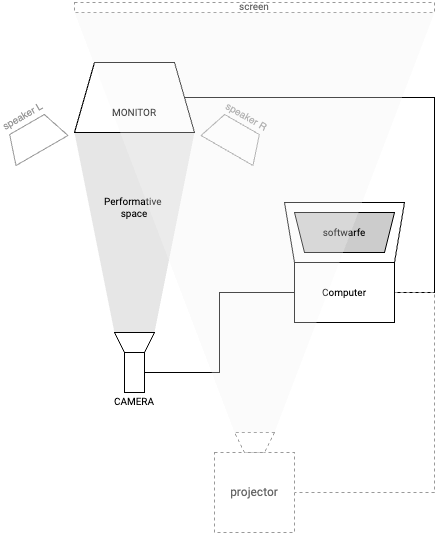
\includegraphics[width=0.8\linewidth]{chapters/appendix/a/image/grapha-videoloop02-2.png}
    \caption{Graphical representation of the \textit{videoloop} system in the digital domain.}
    \label{fig:aa-videoloop-graph02}
\end{figure}
After the first prototype was evaluated and approved, we started refining the Max/MSP software application and selecting the most suitable hardware (screen, camera, and necessary supports).\\
At the software level, we encountered issues synchronising the video and audio data streams in the digital domain. In the original system, video and audio were linked to the tape, recording and playing together. In the digital system, however, the video and audio streams come from different sources with varying sampling rates and buffer sizes (depending on the sound card, the graphic card, and the development environment). In Max/MSP, the video stream is not always captured and played at regular rates (for performance reasons), and delays of a few milliseconds can occur, depending on the graphic card. While this isn’t a problem for real-time visualisation, the delays add up over multiple cycles in the loop and become noticeable after just three loops.\\
We tried different software development environments, such as Touchdesigner (another visual programming language) and Python, to fix this problem. Touchdesigner had the same issues as Max/MSP, while Python introduced new challenges with controlling parameters and maintaining sufficient quality audio and video. As a result, we returned to Max/MSP and developed specific algorithms to offset the delays. Without going into technical details, we designed a custom delay system where video and audio buffers are recorded in dynamic sizes, then synchronised, and played together after a defined time.\\
On the hardware side, the original analogue devices were replaced with modern equipment: the old cathode-ray tube monitor was replaced with a 32” Ultra HD LED screen, and the analogue camera was replaced with a portable 4K camera. The original audio setup, which relied on the camera's built-in microphone and the monitor's speakers, was replaced with a pair of dedicated speakers and a cardioid condenser microphone.\\
After thoroughly evaluating the hardware and software and how they interacted and performed, we successfully created a fully functional digital version of the \textit{videoloop} system. This system was further adjusted and improved during the various iterations based on emerging requirements.

\subsection*{Transmission}
The reactivation of the \textit{videoloop} has been done on five different occasions in three different formats: twice as a video performance (closer to the original), twice as a music performance, and once as an interactive installation.\\
The first reactivation took place as a video performance during Sambin's monographic exhibition at the Castromediano Museum in Lecce on February 19, 2022 (Figures~\ref{fig:aa-iltempoconsuma-lecce01} and ~\ref{fig:aa-iltempoconsuma-lecce02} show the complete stage and a frame from the video created during the exhibition). The second was a music performance at the celebration of the 800th anniversary of the University of Padua, held at Sala Dei Giganti (Palazzo Liviano, Padua) from May 16 to 18, 2022. The third was as an interactive installation during the 2022 edition of Science4All, a science festival at the University of Padua, held every year on September 30. On June 15, 2023, the videoloop was again performed as a music piece during the 19th edition of the Opera Prima Festival in Rovigo, a festival focused on experimental performing arts. The last exhibition was performed as video performance at Cinema Arsenale in Pisa on 20 October 2024, during the \textit{Il Giardino del Video} festival organised by Ondavideo.
\begin{figure}[!h]
    \centering
    \includegraphics[width=\linewidth]{chapters/appendix/a/image/figa-iltempoconsuma-lecce01.png}
    \caption{A screenshot from the audiovisual documentation of the \textit{videoloop} performance at the Castromediano Museum in Lecce.}
    \label{fig:aa-iltempoconsuma-lecce01}
\end{figure}
In all iterations, except for the installation format, the performances included a series of historical works. \textit{Il tempo consuma} was followed by (in different orders each time) \textit{Anche le mani invecchiano}, \textit{Sax}, \textit{Io mi chiamo Michele}, \textit{Auto intervista}, and \textit{Ne…no…}. Notably, the performance does not begin with a blank screen as in the original, but with video documentation of the 1978 version of \textit{Il tempo consuma}. This video gradually fades into the live performance, creating a seamless transition between past and present. Another important shift, in comparison with the original version, is the second screen used in the performance. Originally, a second cathode-ray tube screen was installed above the main one and used to display the camera's direct signal (as shown in Figure~\ref{fig:aa-videoloop-graph01}). In the digital migration, this screen has been replaced with a large projection screen (as shown in Figure~\ref{fig:aa-videoloop-graph02}) behind the performative space, thus behind the main screen (as shown in Figure~\ref{fig:aa-iltempoconsuma-lecce02}).
\begin{figure}[!h]
    \centering
    \includegraphics[width=\linewidth]{chapters/appendix/a/image/figa-iltempoconsuma-lecce02.jpg}
    \caption{\textit{Videoloop} performance stage at the Castromediano Museum in Lecce.}
    \label{fig:aa-iltempoconsuma-lecce02}
\end{figure}
The music performances saw significant development in both the \textit{videoloop} system and its implementation. First, the artist introduced colour (unlike the original black-and-white version), adding a new layer of interaction and experimentation. There was also interaction with the camera and the digital image. On one hand, camera movements, particularly zoom and focus, were used, similar to previous works by the artist, such as \textit{VTR\&I}. On the other hand, controls for RGB colour, saturation, and brightness were introduced for the digital image. These adjustments allowed the artist to explore new performative pathways with the \textit{videoloop} system. Additionally, a vocal performer was included, using the \textit{videoloop} to create layered audio textures, often in relation to the video.\\
\begin{figure}[!h]
    \centering
    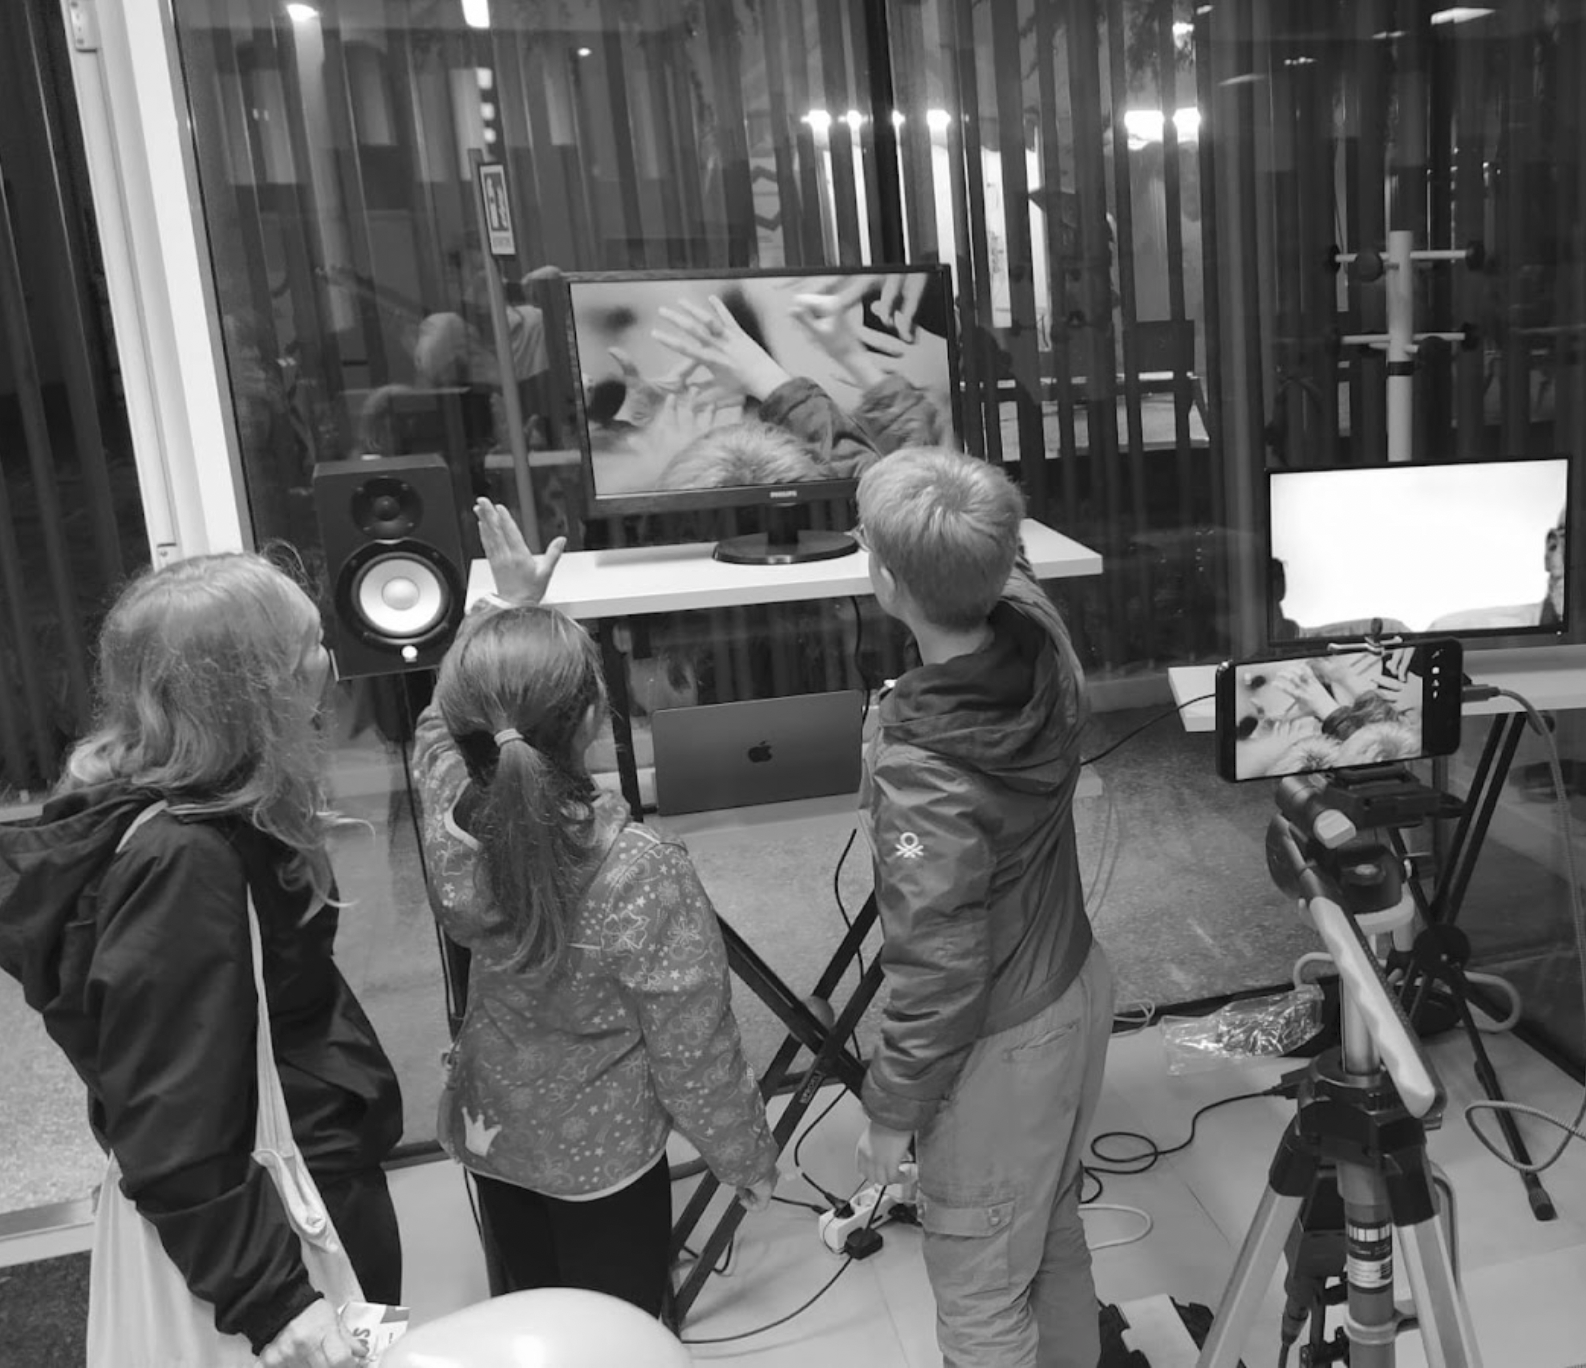
\includegraphics[width=\linewidth]{chapters/appendix/a/image/figa-iltempoconsuma-installation.png}
    \caption{A photo from the interactive installation set-up of the \textit{videoloop} at the Science4All festival in Padua.}
    \label{fig:aa-iltempoconsuma-installation}
\end{figure}
In the interactive installation format (seen in Figure~\ref{fig:aa-iltempoconsuma-installation}), the \textit{videoloop} implementation was straightforward, consisting of a loop that ran continuously throughout the installation. However, there were some technological modifications, such as using a smartphone camera to transmit the video stream via Wi-Fi. The same camera system was used also during the last video performance in Figure~\ref{fig:aa-iltempoconsuma-pisa}.
\begin{figure}[!h]
    \centering
    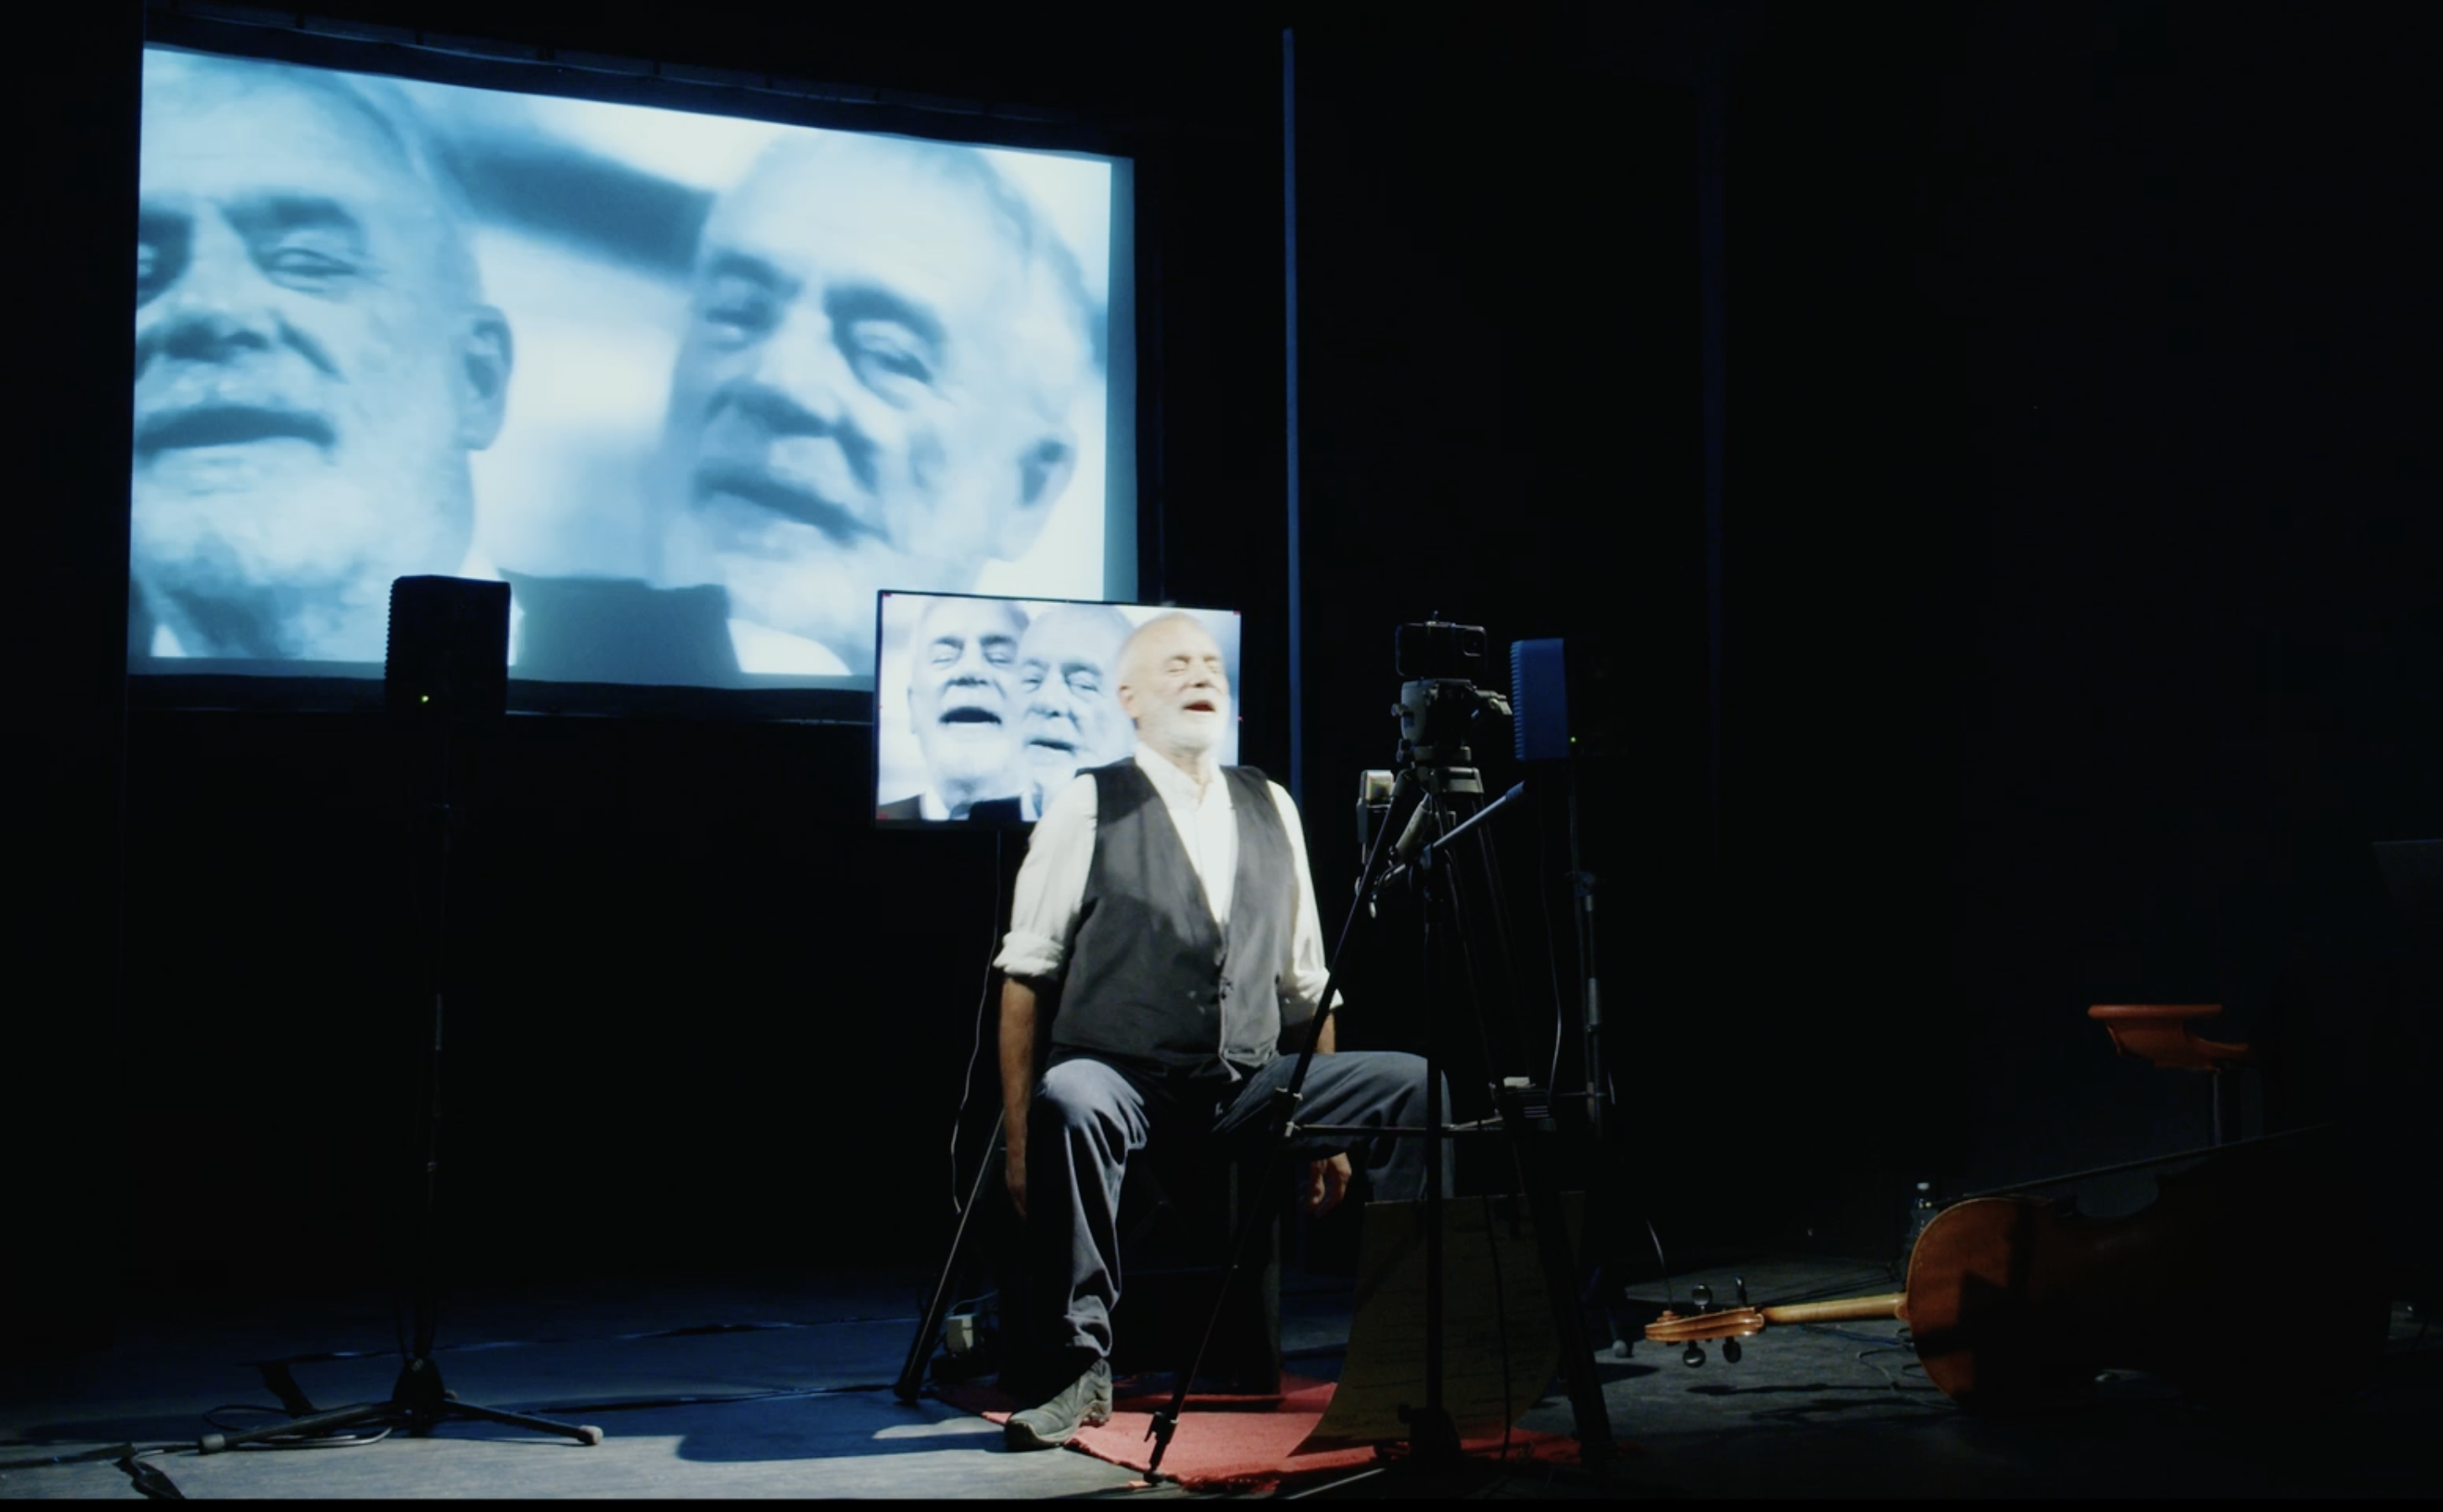
\includegraphics[width=\linewidth]{chapters/appendix/a/image/figa-iltempoconsuma-pisa.png}
    \caption{A screenshot from the audiovisual documentation of the \textit{videoloop} performance at the Cinema Arsenale in Pisa.}
    \label{fig:aa-iltempoconsuma-pisa}
\end{figure}

\subsection*{Archiving}
For each iteration, \textit{bit}s, \textit{data}, and \textit{experience}s were stored and organised as separate \textit{Iteration Files} (IFs). The new hardware and software components represent the \textit{bit}s, which remain mostly unchanged across different implementations. Still, they are entirely different from the original version and slightly altered in the installation version. Because of this, we also had to revise some of the \textit{data} related to the original version (like the relationship between hardware and software, the roles of elements, operating instructions, etc.) since we needed to change certain instructions and parts of the performative actions based on the new \textit{bit}s. Much documentation capturing the experience and the look of the digital reactivation was produced during the rehearsal and prototyping phases and the performances. Figure~\ref{fig:aa-graph_mdc} show graphical approximation of the archived artwork \textit{Il tempo consuma} through the MDC model. Chapter~\ref{ch:4-madc_model_application} show how the MDC model has been applied using the graphical database Neo4j in order to archive the entire \textit{videoloop} performances.

\section{Data compilation}
According to the \textit{data} compilation, i.e. instruction template and BVL application, introduced in Chapter~\ref{ch:3-mdc_model-reactivation_workflow-instruction_template} and \ref{ch:4-madc_model_application}, we report some of the most essential parts of the technical instructions and mappings. \textit{Data} compilation was fundamental to this performance. During the various iterations, many technicians (sound engineers, video technicians, electricians, etc.) set the \textit{videoloop} up in different stages. In order to have all the technical requirements, a tech rider (which is nothing but a set of information, instructions and requirements) is usually helpful to share before staging with all the people involved. Here, we report part of the tech rider of just video performance format and include the \textit{bits lists and specifications}, the stage plan (\textit{spatial mapping}), the routing (the \textit{physical implementation mapping}), and the \textit{graphical information}. We add some details (which are not included in the tech rider) about the \textit{conceptual} and \textit{process mappings}. Furthermore, in this particular case, Michele Sambin also created a \textit{temporal mapping} for each performance. The \textit{temporal mappings} comprehend hand-drawn textual and graphical information about the action during the performance.

\subsection*{Bit lists and specifications}
The table reports the list of bits divided by \textit{hardware}, \textit{software}, \textit{audiovisuals}, and \textit{musical instruments}, with the related specifications and requirements.

\begin{longtable}{|p{0.3\textwidth}|p{0.05\textwidth}|p{0.55\textwidth}|}
    \caption{Hardware} \label{tab:a-data-hardware} \\
    \hline
    \textbf{Name} & \textbf{Q} & \textbf{Specification and notes} \\
    \hline
    Full-range loudspeaker & 4 & \scriptsize with adjustable height stands. \\
    \hline
    Audio mixer & 1 & \scriptsize 4 Input / 4 Output / 2 Aux. \\
    \hline
    Sound Card & 1 & \scriptsize 2 In / 2 Out. \\
    \hline
    Laptop & 1 & \scriptsize macOS > v.11.6 (3 HDMI output). \\
    \hline
    Microphone A & 1 & \scriptsize NEUMANN KMS105 (condenser-super-cardioid). With a high stand ($\simeq$2 meters). \\
    \hline
    Microphone B & 1 & \scriptsize Clip Violoncello. \\
    \hline
    Monitor A & 1 & \scriptsize The monitor is positioned on a dedicated stand at the performers' face height.\\
    \hline
    Monitor B & 1 & \scriptsize Monitor LCD 7"/11". The monitor is positioned below the camera and facing the performers. It works as a visual feedback for the performer.\\
    \hline
    Screen C & 1 & \scriptsize Projection screen (4 meters at the base). The screen must be raised from the ground by approximately 50 cm; the projection is in 16/9.\\
    \hline
    Projector & 1 & \scriptsize 8000 ansi lumen. The optics should be calculated according to the distance to the screen.\\
    \hline
    LED bar & 1 & \scriptsize 1 meter. The LED bar is positioned above the performer (2m) - parallel to the floor - with a high stand.\\
    \hline
    Camera & 1 & \scriptsize Blackmagic Poket Cinema / obiettivo zoom 14-140.\\
    \hline
    USB C to HDMI Adaptor & 3 & \scriptsize \\
    \hline
    Overhead Microphone Stand & 1 & \scriptsize Height >= 2m.\\
    \hline
    LED bar stand  & 1 & \scriptsize Height >= 2m. The stand could be an overhead microphone stand. \\
    \hline
    Speaker stand   & 4 & \scriptsize With adjustable height.\\
    \hline
    LCD stand & 1 & \scriptsize Adjustable height stand for the Monitor LCD 32".\\
    \hline
\end{longtable}

\begin{longtable}{|p{0.3\textwidth}|p{0.6\textwidth}|}
    \caption{Software} \label{tab:a-data-software} \\
    \hline
    \textbf{Name} & \textbf{Specification and notes} \\
    \hline
    Max/MSP & \scriptsize Version >= 8. \\
    \hline
    Videoloop application software & \scriptsize A folder containing all the Max/MSP Patches for running the application software. \\
    \hline
\end{longtable}

\begin{longtable}{|p{0.4\textwidth}|p{0.5\textwidth}|}
    \caption{Audiovisual} \label{tab:a-data-audiovisual} \\
    \hline
    \textbf{Name} & \textbf{Specification and notes} \\
    \hline
    1978iltempoconsuma.mp4 & \scriptsize The digital version of the original audiovisual documentation of the 1978 performance of \textit{Il tempo consuma} by Michele Sambin. \\
    \hline
\end{longtable}

\begin{longtable}{|p{0.3\textwidth}|p{0.05\textwidth}|p{0.55\textwidth}|}
    \caption{Various (Musical instrument)} \label{tab:a-data-various} \\
    \hline
    \textbf{Name} & \textbf{Q} & \textbf{Specification and notes} \\
    \hline
    Cello & 1 & \scriptsize \\
    \hline
    Sax soprano & 1 & \scriptsize \\
    \hline
    clarinet & 1 & \scriptsize \\
    \hline
\end{longtable}

\subsection*{Spatial mapping}
Figure~\ref{fig:aa-mapping-spatial} shows the stage plan of the \textit{videoloop}, i.e. how the hardware and performers are arranged in the space of the performance. For the different implementations, the stage plan slightly differs. Here, we represent the basic one, i.e. the video performance format.

\begin{figure}[!h]
    \centering
    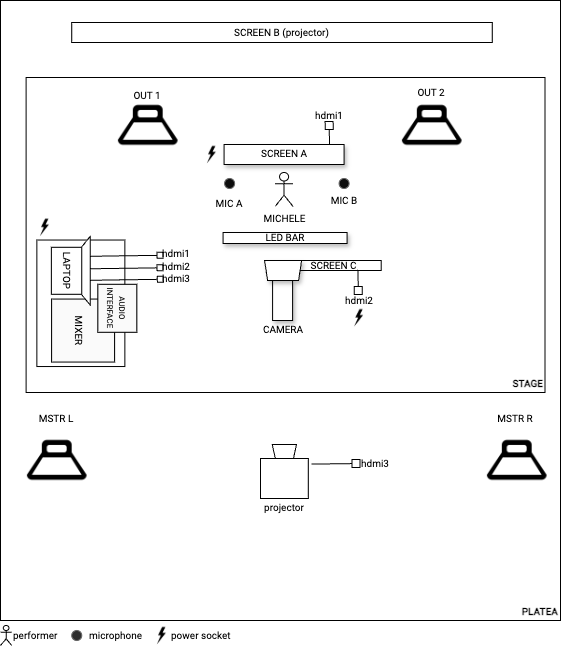
\includegraphics[width=\linewidth]{chapters/appendix/a/image/grapha-data-space.png}
    \caption{Stage plan (\textit{spatial mapping}) of the \textit{videoloop} video performance}
    \label{fig:aa-mapping-spatial}
\end{figure}

\subsection*Conceptual mapping}
Figure~\ref{fig:aa-mapping-conceptual} shows the conceptual mapping of the \textit{videoloop} according to the BVL. The produced effect, the focus of this performance, is the performative space created between the camera –which records what happens in front of the display–and the display itself–which plays what the camera records after 24 seconds. The performer interacts with this space by producing performative actions inside this ``real space.''

\begin{figure}[!h]
    \centering
    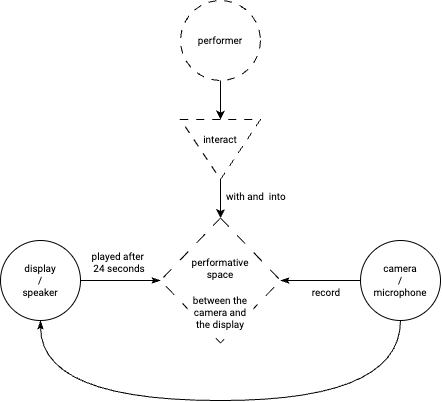
\includegraphics[width=0.75\linewidth]{chapters/appendix/a/image/grapha-data-concept.png}
    \caption{\textit{Conceptual mapping} of the \textit{videoloop} through the BVL.}
    \label{fig:aa-mapping-conceptual}
\end{figure}

\subsection*{Physical implementation mapping}
Figure~\ref{fig:aa-mapping-physical} shows a physical implementation of the entire videoloop using the BVL. This mapping shows how the individual \textit{bit}s should be linked together and interact between them.

\begin{figure}[!h]
    \centering
    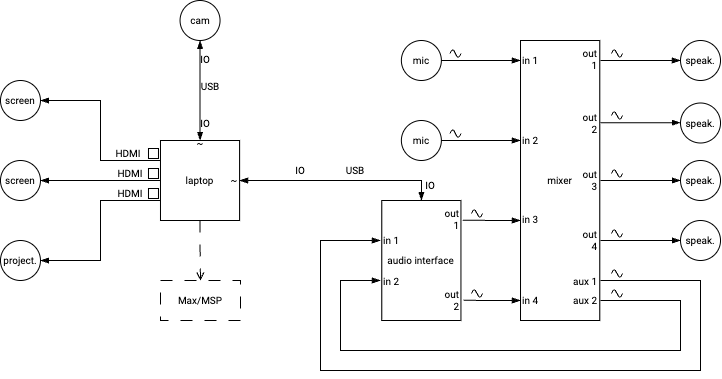
\includegraphics[width=\linewidth]{chapters/appendix/a/image/grapha-data-physical.png}
    \caption{\textit{Physical implementation mapping} of the \textit{videoloop} with the BVL. Link and interaction between \textit{bit}s.}
    \label{fig:aa-mapping-physical}
\end{figure}

\subsection*{Process mapping}
Figure~\ref{fig:aa-mapping-process} reports the highest level of Max/MSP’s \textit{videoloop} application software. Here, the custom delay for synchronising audio and video is summarised. A counter that runs at an fps rate controls and synchronises the delay. 

\begin{figure}[!h]
    \centering
    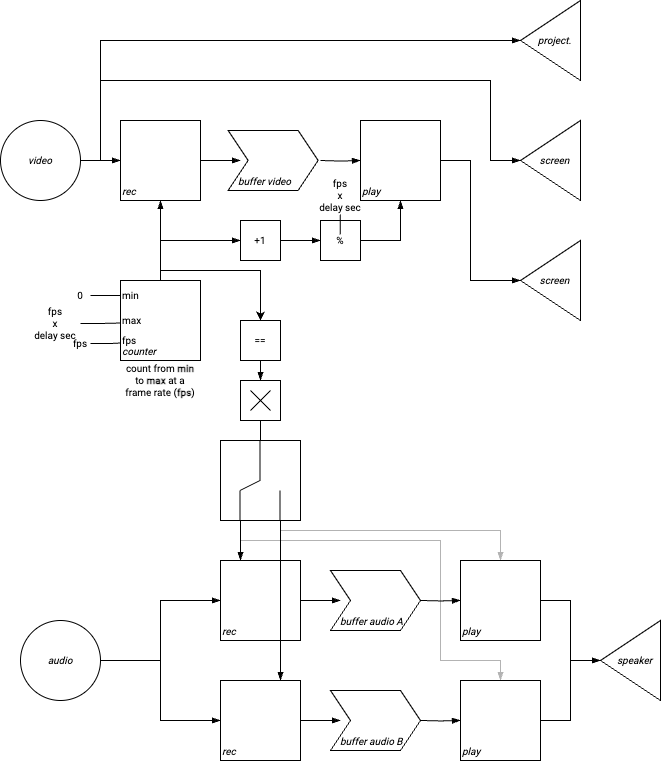
\includegraphics[width=0.85\linewidth]{chapters/appendix/a/image/grapha-data-process.png}
    \caption{\textit{Process mapping} of the Max/MSP’s \textit{videoloop} software application at the highest level.}
    \label{fig:aa-mapping-process}
\end{figure}

\subsection*{Temporal mappings}
Figures~\ref{fig:aa-mapping-temporal-01a} and \ref{fig:aa-mapping-temporal-01b} (at the end of the chapter) show the temporal mapping for the musical performance at Sala Dei Giganti (Palazzo Liviano, Padua) on May 16, 2022. Figure \ref{fig:aa-mapping-temporal-02} shows the temporal mapping for the last video performance.

\subsection*{Graphical information}
Figure~\ref{fig:aa-mapping-graphical} shows a picture that informs about the dispositions of the \textit{bit}s (identified with some text) and an example of the stage's appearance.

\begin{figure}[!h]
    \centering
    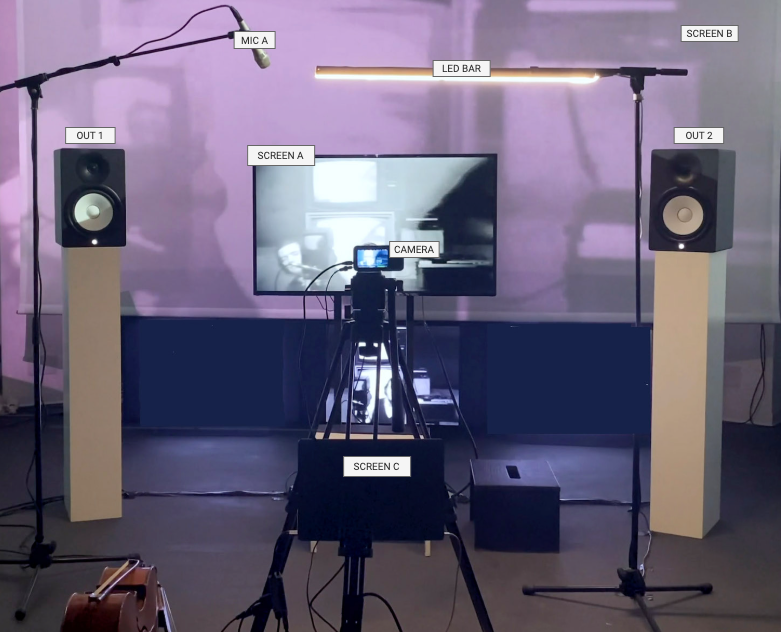
\includegraphics[width=\linewidth]{chapters/appendix/a/image/grapha-data-graphic.png}
    \caption{Graphical information for the \textit{bit}s’ placement and stage appearance.}
    \label{fig:aa-mapping-graphical}
\end{figure}

\section{Discussion}
The digital migration of the \textit{videoloop} has inevitable differences compared with the original. The first differentiation regards the composition of the whole system. Figure~\ref{fig:aa-videoloop-graph02} shows that digital technologies allow for significant hardware streamlining, consequently lightening the system. So, even the required actions undergo a relevant transformation and simplification. The original version required a coordinated and delicate operation to activate the loop. At the beginning of every performance, two people had to turn the two video recorders on simultaneously. In doing so, the likelihood of errors was significant, and if something went wrong, they had to restart the system all over again by rewinding the tape. With the build-on-purpose software we developed, activating the loop requires only one person. The software also provides an OSC system and can be operated by different control devices connected wirelessly to it. The performer can potentially control the system by himself, using an OSC application for mobile devices.\\
Although these digital transformations appear highly advantageous, they directly result in an appearance transformation of the artwork. The produced effect of this \textit{videoloop} technique is the video and sound feedback that leads to the degradation of both components. The side effect of digital migration is particularly noticeable in the video domain. For each loop cycle, areas above a specific brightness threshold shift toward white, while those below towards black. Screen and camera settings and the brightness of the performance space define the brightness threshold, which is particularly difficult to control. In the digital version, the same variables determine the number of cycles the system takes to reach a saturation stage. The saturation state is due to the nature of the pixels, which are the components of the digital system. The degradation process is an aesthetic element we can define as ``image error'' \cite{Gfeller2013-je}, a particularly popular effect in video art in the 1970s. Since the ``image error'' results from the ``wrong'' use of a specific device, the effect is specifically related to that device. Consequently, technological migration leads to consistent changes in error production. Therefore, we obtain an unavoidable transformation of the visual degradation process compared to the original artwork. Figure~\ref{fig:aa-videoloop-comparison} shows a comparison between the analogue and digital versions. As we can see, in both cases, the degradation process highlights the image's generative nature: the cathode-ray tube's scan lines and the LCD screen pixels (that cause the saturation effect).

\begin{figure}[!h]
    \centering
    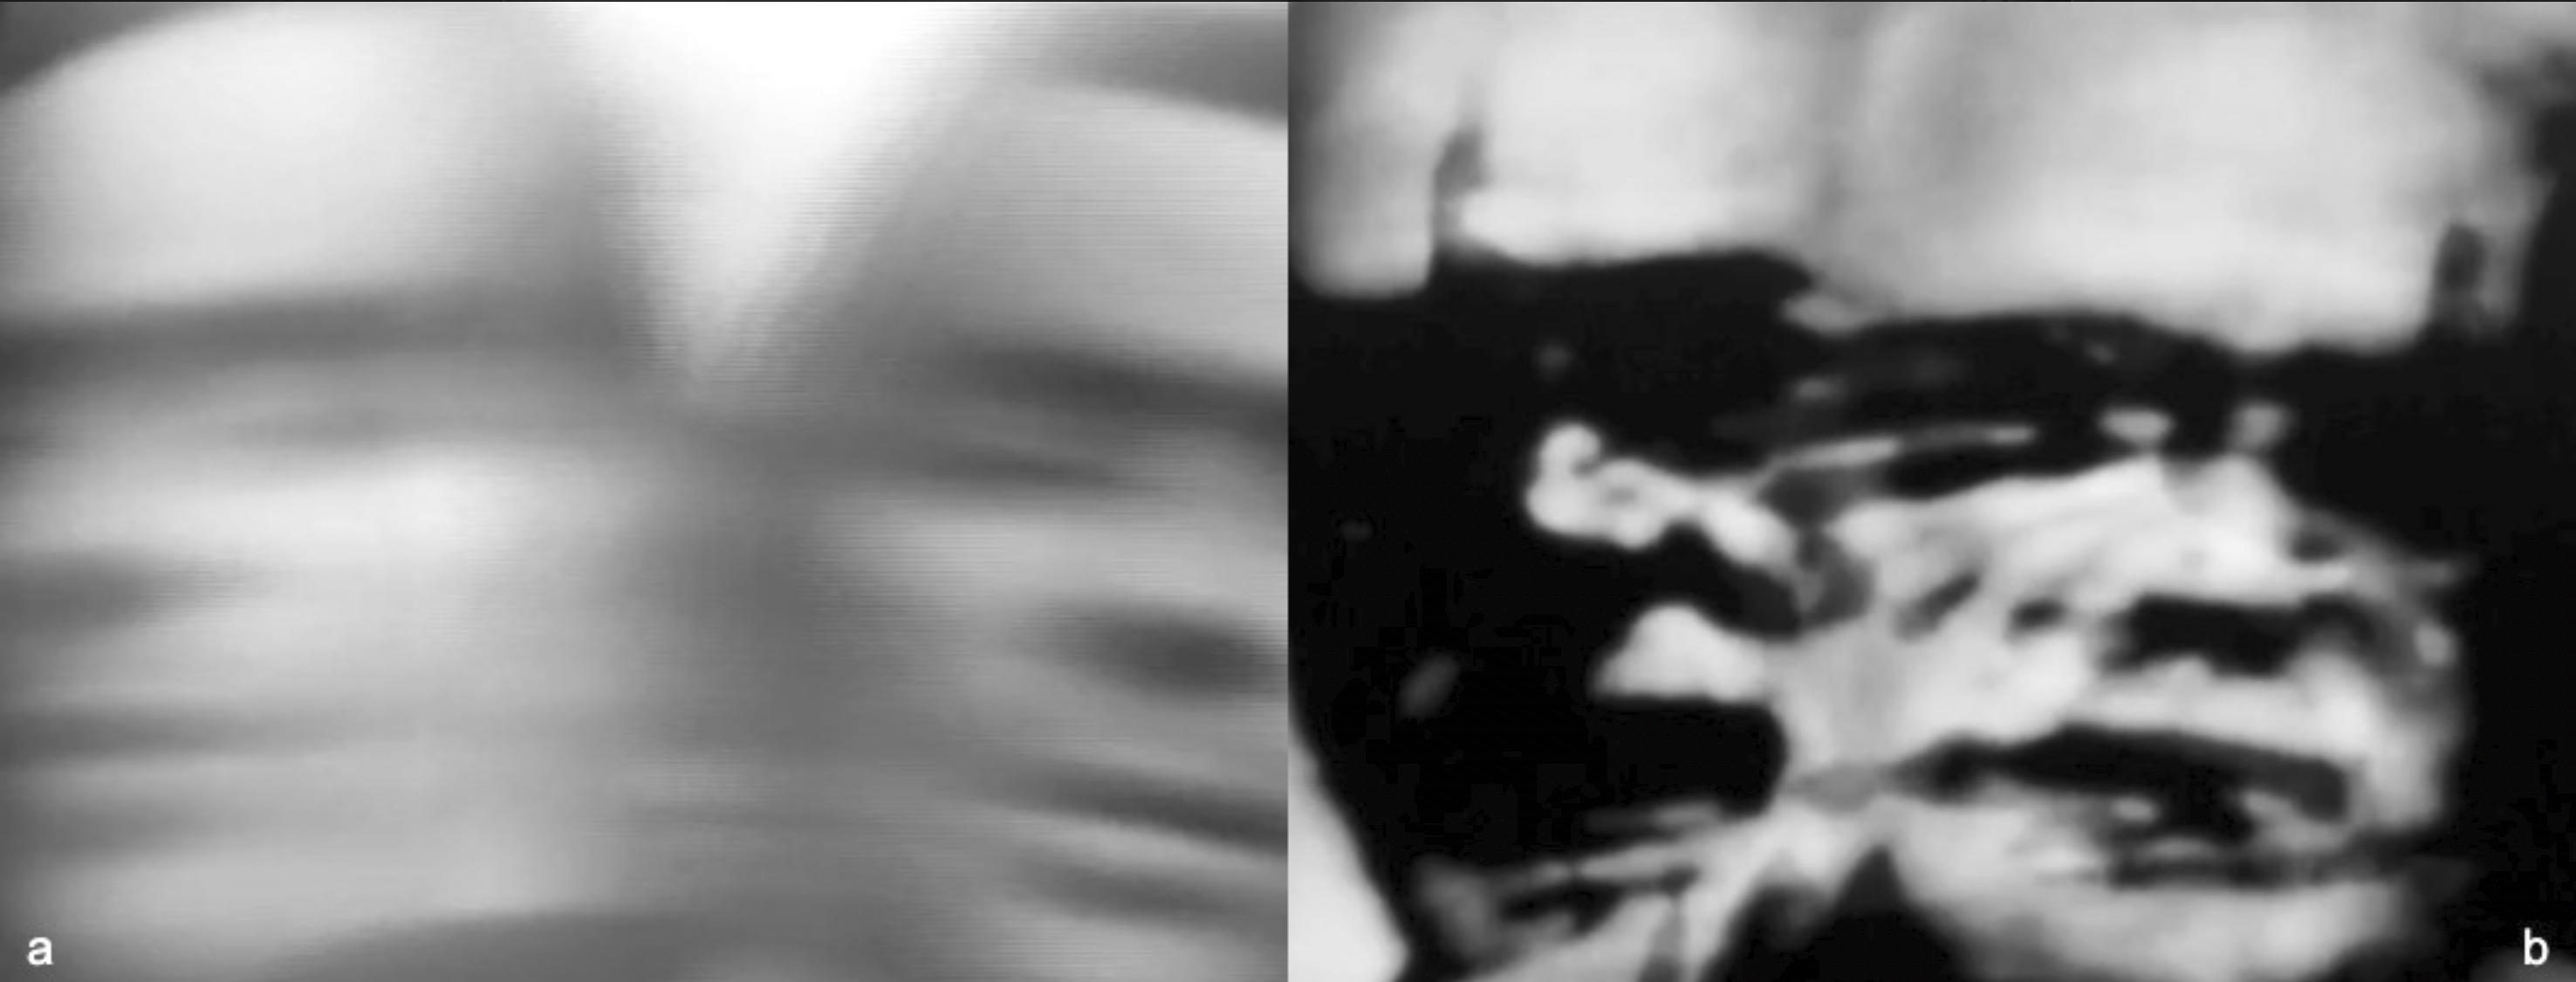
\includegraphics[width=\linewidth]{chapters/appendix/a/image/figa-videoloop-comparison.jpg}
    \caption{Figure 14 Comparison between the ``image error'' (or image degradation) in the analogue (a) and digital (b) versions.}
    \label{fig:aa-videoloop-comparison}
\end{figure}

However, as mentioned, the artist does not define his work by its visual result but rather by the possibilities created within the performative space (the ``real space'') between the camera and the screen. This space is crucial because it initiates a dialogue between the performer and their repeated, accumulating, and degrading reproductions every 24 seconds. The key element is this interaction with the past and its degradation over time. What matters is not the material aspect of the degradation but the process itself—the time consumes.\\
In the conceptual mapping, we defined the performative space where the performer acts as the outcome of the artwork. The goal of conceptual mapping is to combine and summarise all the information about the work (\textit{bit}s, \textit{data}, and \textit{experience}s) in a way that goes beyond the specific medium, getting as close as possible to the concept and the experience generated by the work. This conceptual mapping is essential, especially in technological migration cases, as it should be the constant element that remains unchanged between the original and its reactivation.\\

\begin{figure}[!h]
    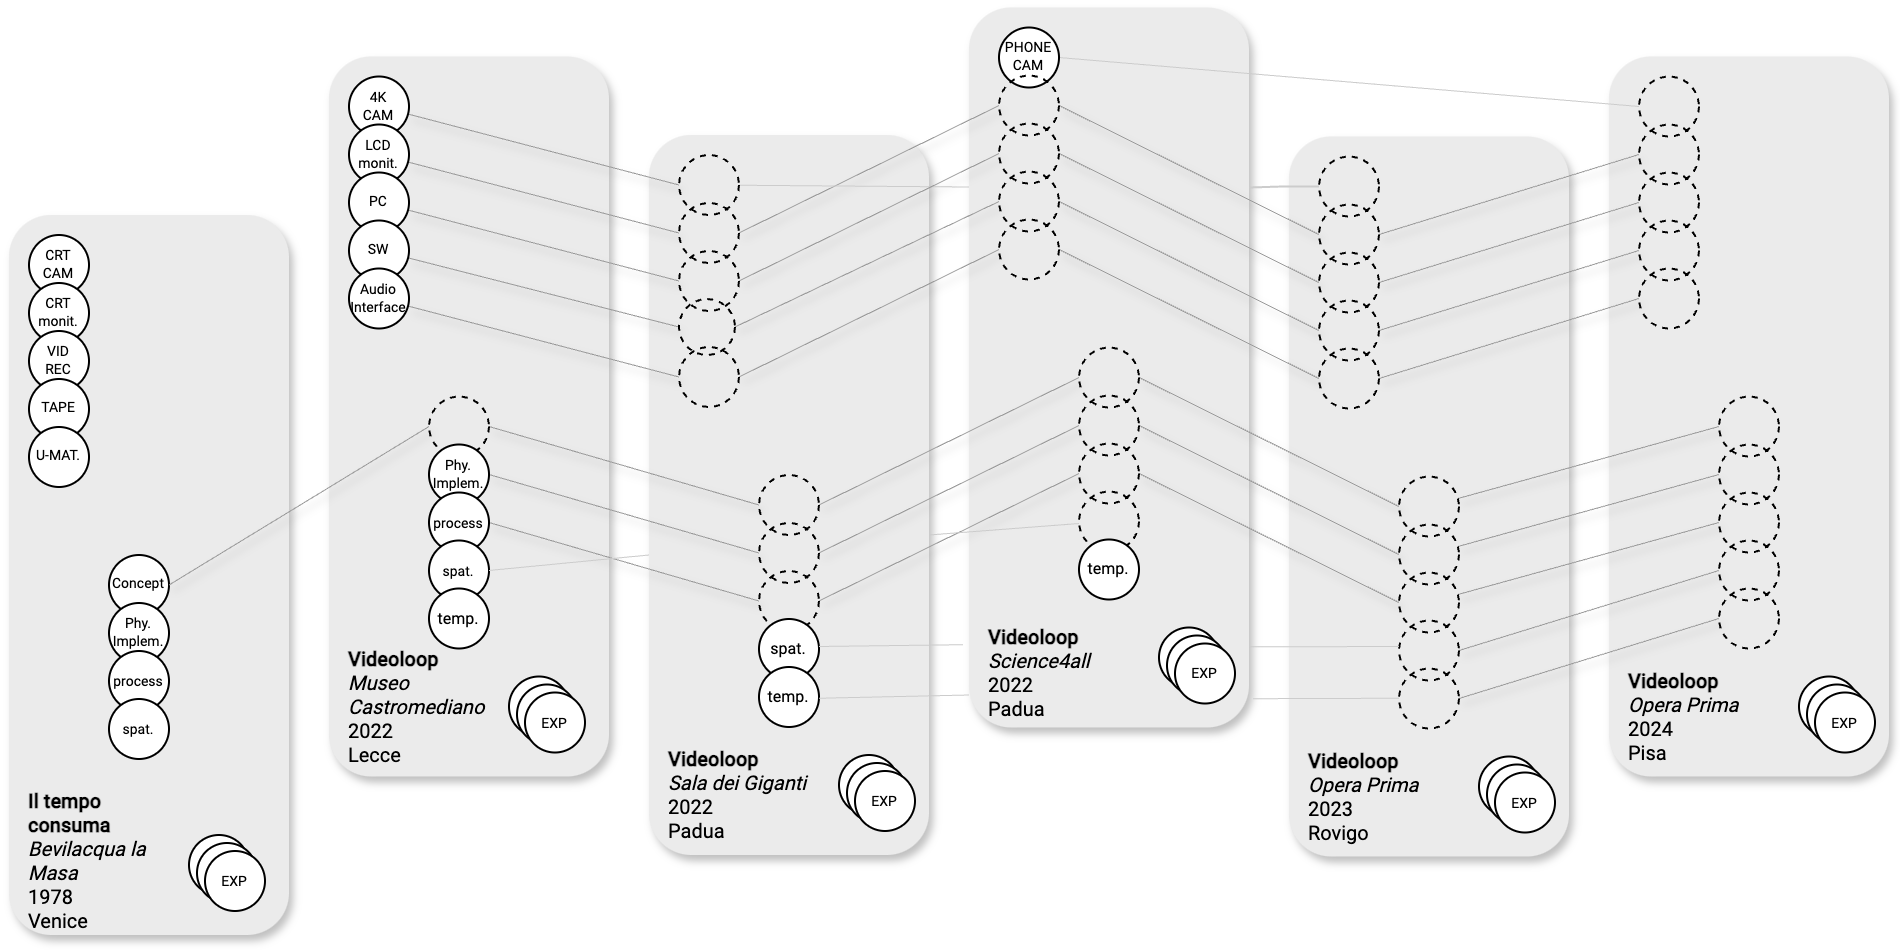
\includegraphics[width=\linewidth]{chapters/appendix/a/image/grapha-mdc.png}
    \caption{Approximate chronological representation of \textit{Il tempo consuma} through the MDC. The chronological representation show how the \textit{conceptual mapping} remain unchanged from 1978 to the present.}
    \label{fig:aa-graph_mdc}
\end{figure}

Figure~\ref{fig:aa-graph_mdc} shows an approximate representation of \textit{Il tempo consuma} through the \textit{Multilevel Dynamic Conservation} (MDC) Model. This representation clearly shows how the model records the artwork's dynamic authenticity and unfolding identity through multiple belongingness (represented by arrows between the IFs). 
However, the \textit{videoloop} reactivation is also a particular case study since the same reactivation belongs not only to the artwork \textit{Il tempo consuma} but to a series of artworks made with such a technique. So the reactivation’s IFs form part of the \textit{Iteration Series} of those pieces reproduced during the \textit{videoloop} performance, such as \textit{Anche le mani invecchiano}, \textit{Autointervista}, \textit{Ne..No..}, and \textit{Io mi chiamo Michele}. As shown in Figure~\ref{fig:c4-neo4j-multipleartworks} on Chapter~\ref{ch:4-madc_model_application} the MDC model also allows multiple belongingness for entire IFs.



\begin{figure}
    \centering
    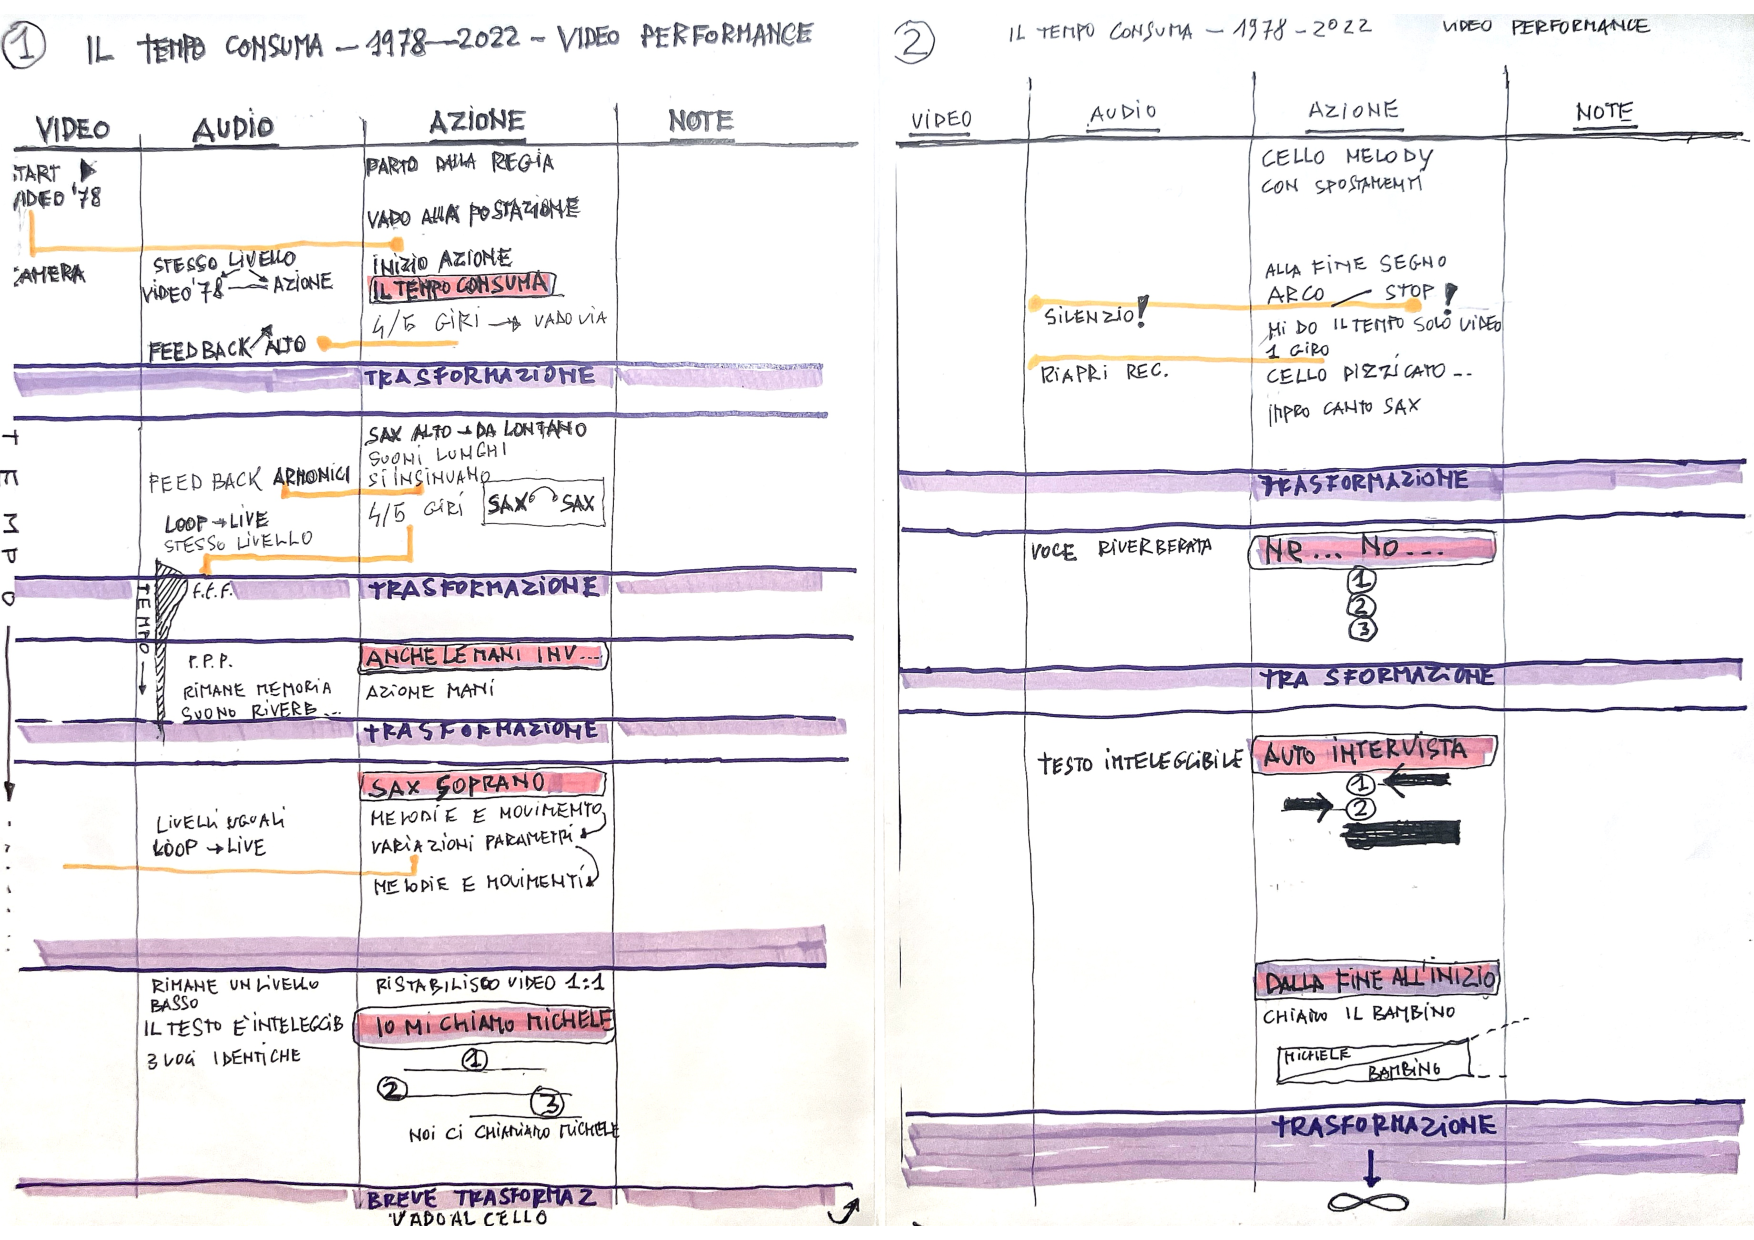
\includegraphics[height=\linewidth, angle=90]{chapters/appendix/a/image/figa-data-temporal01a.pdf}
    \caption{\textit{Temporal mapping}–part 1–for the musical \textit{videoloop} performance at Sala Dei Giganti (Palazzo Liviano, Padua) on May 16, 2022.}
    \label{fig:aa-mapping-temporal-01a}
\end{figure}

\begin{figure}
    \centering
    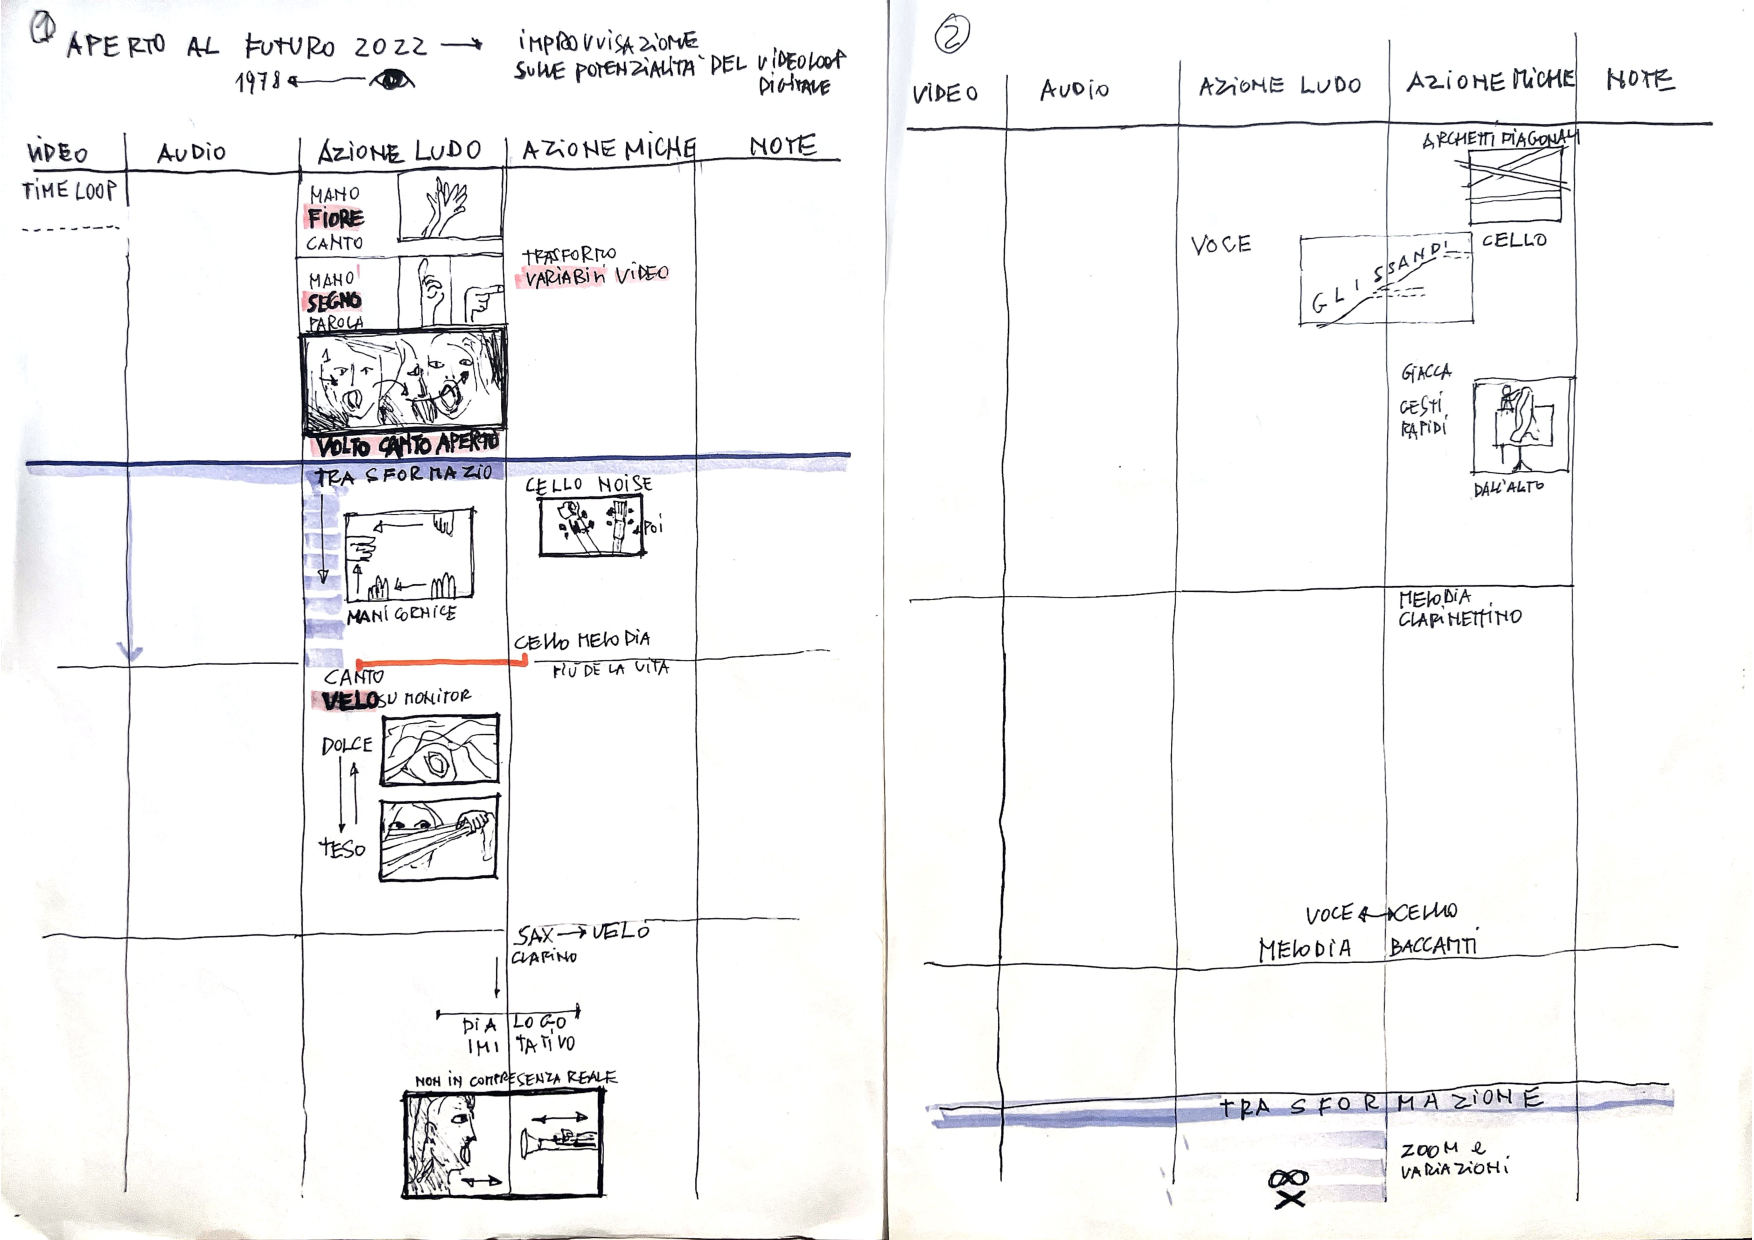
\includegraphics[height=\linewidth, angle=90]{chapters/appendix/a/image/figa-data-temporal01b.pdf}
    \caption{\textit{Temporal mapping}–part 2–for the musical \textit{videoloop} performance at Sala Dei Giganti (Palazzo Liviano, Padua) on May 16, 2022.}
    \label{fig:aa-mapping-temporal-01b}
\end{figure}

\begin{figure}
    \centering
    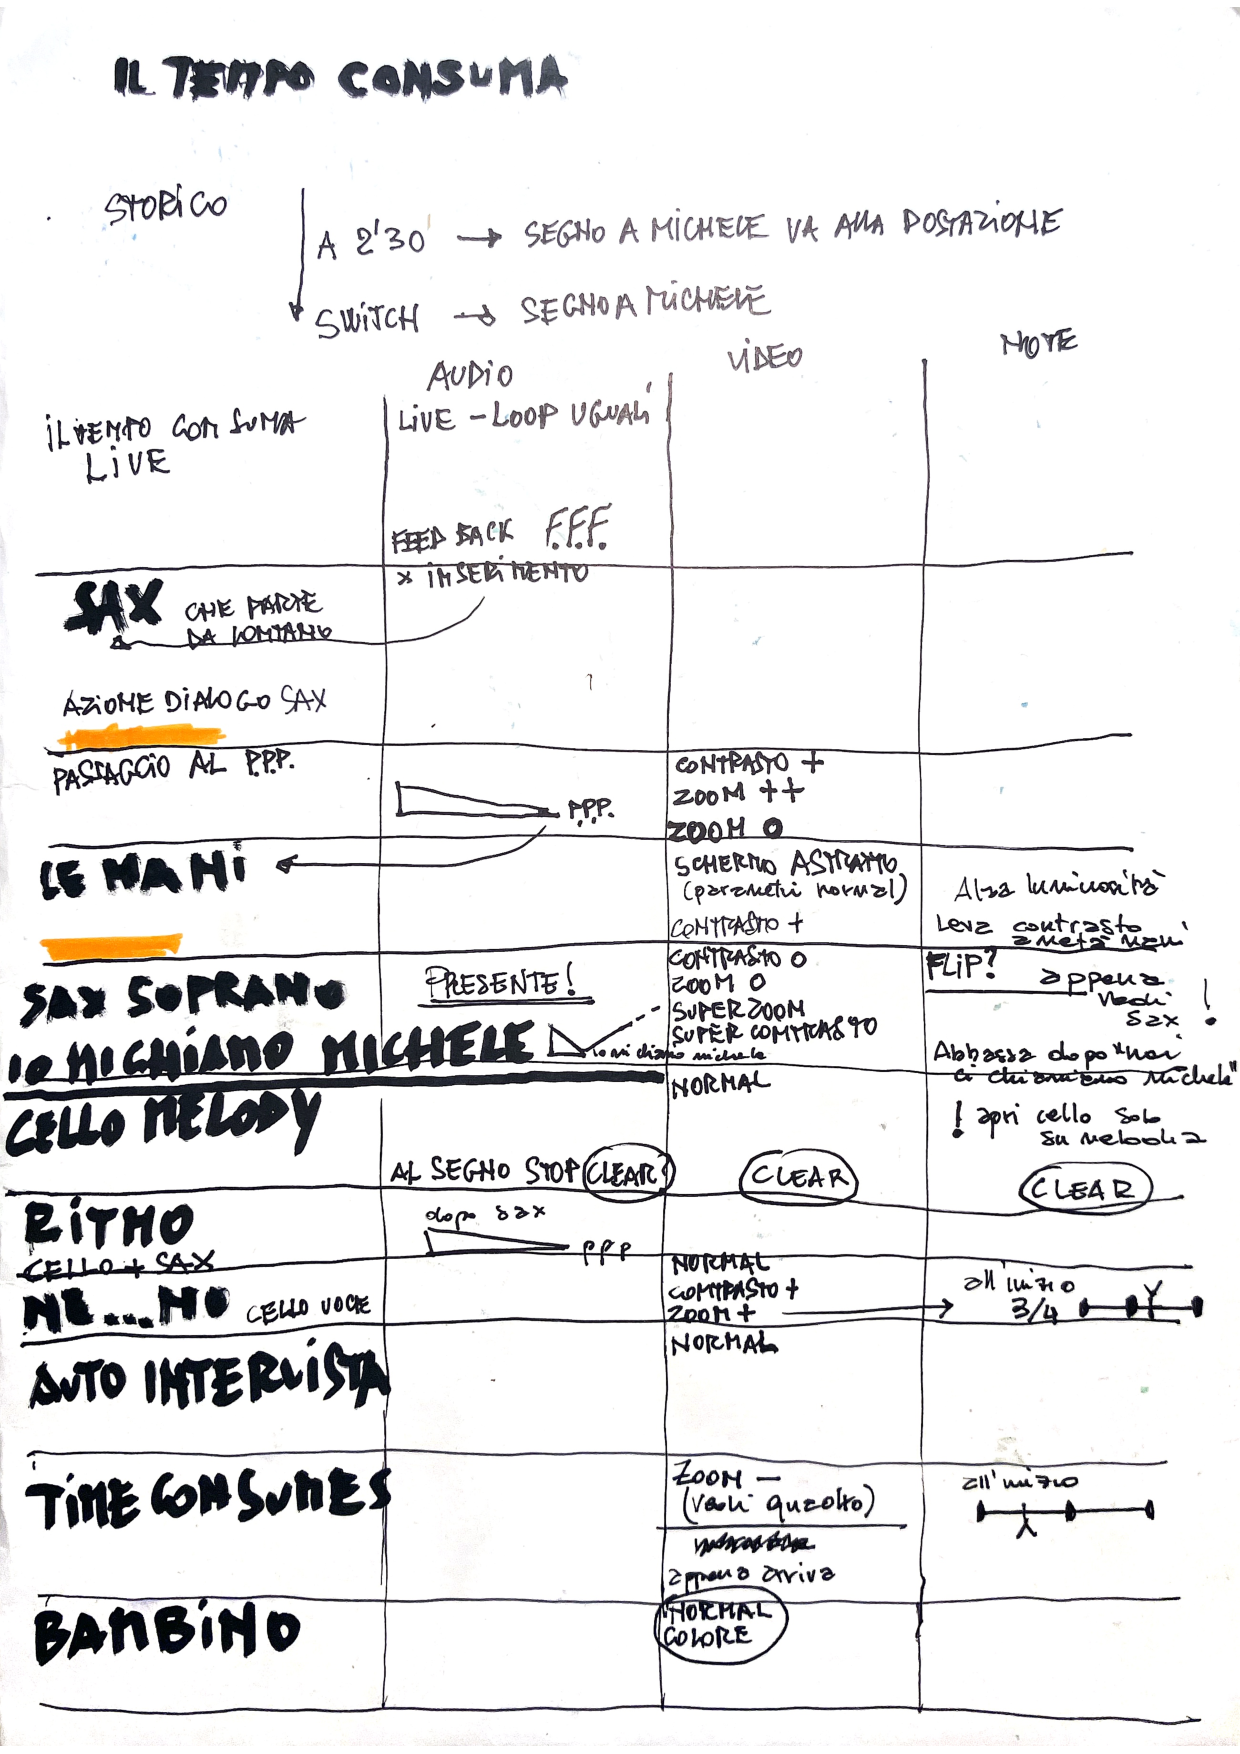
\includegraphics[width=\linewidth]{chapters/appendix/a/image/figa-data-temporal02.pdf}
    \caption{\textit{Temporal mapping} for the \textit{videoloop} performance at Cinema Arsenale in Pisa on October 20, 2024.}
    \label{fig:aa-mapping-temporal-02}
\end{figure}

